% Created by tikzDevice version 0.10.1 on 2016-09-07 19:08:02
% !TEX encoding = UTF-8 Unicode
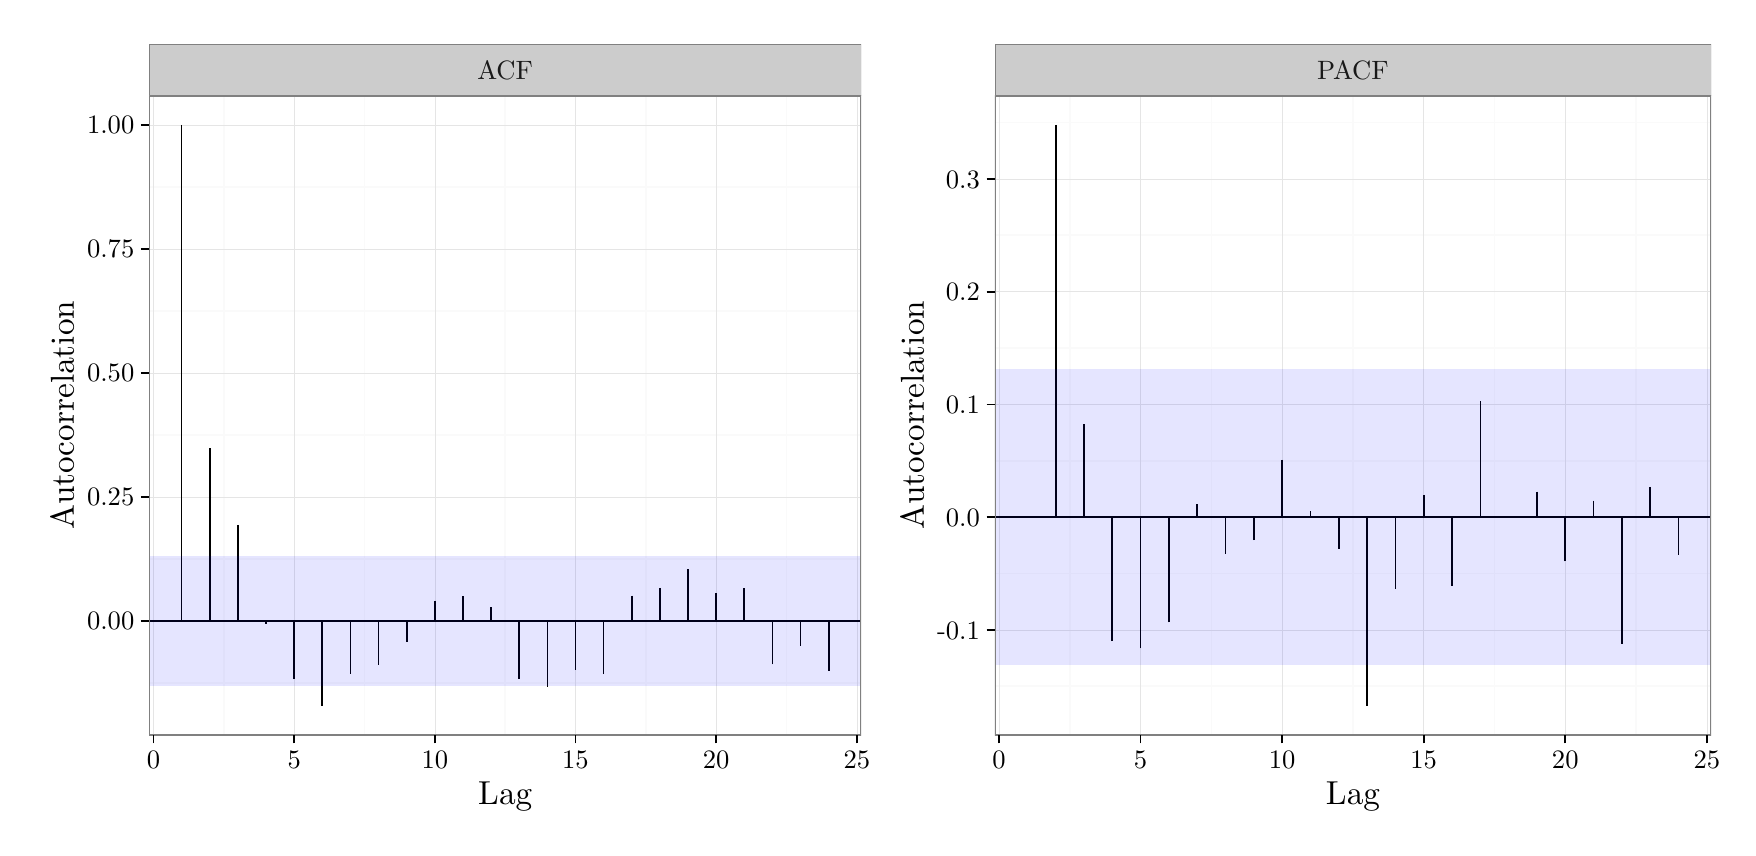
\begin{tikzpicture}[x=1pt,y=1pt]
\definecolor{fillColor}{RGB}{255,255,255}
\path[use as bounding box,fill=fillColor,fill opacity=0.00] (0,0) rectangle (614.29,289.08);
\begin{scope}
\path[clip] (  0.00,  0.00) rectangle (307.15,289.08);
\definecolor{drawColor}{RGB}{255,255,255}
\definecolor{fillColor}{RGB}{255,255,255}

\path[draw=drawColor,line width= 0.6pt,line join=round,line cap=round,fill=fillColor] ( -0.00,  0.00) rectangle (307.15,289.08);
\end{scope}
\begin{scope}
\path[clip] ( 43.93, 33.48) rectangle (301.15,264.47);
\definecolor{fillColor}{RGB}{255,255,255}

\path[fill=fillColor] ( 43.93, 33.48) rectangle (301.15,264.47);
\definecolor{drawColor}{gray}{0.98}

\path[draw=drawColor,line width= 0.6pt,line join=round] ( 43.93, 52.35) --
	(301.15, 52.35);

\path[draw=drawColor,line width= 0.6pt,line join=round] ( 43.93, 97.15) --
	(301.15, 97.15);

\path[draw=drawColor,line width= 0.6pt,line join=round] ( 43.93,141.96) --
	(301.15,141.96);

\path[draw=drawColor,line width= 0.6pt,line join=round] ( 43.93,186.76) --
	(301.15,186.76);

\path[draw=drawColor,line width= 0.6pt,line join=round] ( 43.93,231.57) --
	(301.15,231.57);

\path[draw=drawColor,line width= 0.6pt,line join=round] ( 70.87, 33.48) --
	( 70.87,264.47);

\path[draw=drawColor,line width= 0.6pt,line join=round] (121.70, 33.48) --
	(121.70,264.47);

\path[draw=drawColor,line width= 0.6pt,line join=round] (172.54, 33.48) --
	(172.54,264.47);

\path[draw=drawColor,line width= 0.6pt,line join=round] (223.37, 33.48) --
	(223.37,264.47);

\path[draw=drawColor,line width= 0.6pt,line join=round] (274.21, 33.48) --
	(274.21,264.47);
\definecolor{drawColor}{gray}{0.90}

\path[draw=drawColor,line width= 0.2pt,line join=round] ( 43.93, 74.75) --
	(301.15, 74.75);

\path[draw=drawColor,line width= 0.2pt,line join=round] ( 43.93,119.56) --
	(301.15,119.56);

\path[draw=drawColor,line width= 0.2pt,line join=round] ( 43.93,164.36) --
	(301.15,164.36);

\path[draw=drawColor,line width= 0.2pt,line join=round] ( 43.93,209.16) --
	(301.15,209.16);

\path[draw=drawColor,line width= 0.2pt,line join=round] ( 43.93,253.97) --
	(301.15,253.97);

\path[draw=drawColor,line width= 0.2pt,line join=round] ( 45.45, 33.48) --
	( 45.45,264.47);

\path[draw=drawColor,line width= 0.2pt,line join=round] ( 96.29, 33.48) --
	( 96.29,264.47);

\path[draw=drawColor,line width= 0.2pt,line join=round] (147.12, 33.48) --
	(147.12,264.47);

\path[draw=drawColor,line width= 0.2pt,line join=round] (197.95, 33.48) --
	(197.95,264.47);

\path[draw=drawColor,line width= 0.2pt,line join=round] (248.79, 33.48) --
	(248.79,264.47);

\path[draw=drawColor,line width= 0.2pt,line join=round] (299.62, 33.48) --
	(299.62,264.47);
\definecolor{drawColor}{RGB}{0,0,0}

\path[draw=drawColor,line width= 0.6pt,line join=round] ( 43.93, 74.75) -- (301.15, 74.75);

\path[draw=drawColor,line width= 0.6pt,line join=round] ( 55.62,253.97) -- ( 55.62, 74.75);

\path[draw=drawColor,line width= 0.6pt,line join=round] ( 65.79,137.12) -- ( 65.79, 74.75);

\path[draw=drawColor,line width= 0.6pt,line join=round] ( 75.95,109.43) -- ( 75.95, 74.75);

\path[draw=drawColor,line width= 0.6pt,line join=round] ( 86.12, 73.75) -- ( 86.12, 74.75);

\path[draw=drawColor,line width= 0.6pt,line join=round] ( 96.29, 53.64) -- ( 96.29, 74.75);

\path[draw=drawColor,line width= 0.6pt,line join=round] (106.45, 43.98) -- (106.45, 74.75);

\path[draw=drawColor,line width= 0.6pt,line join=round] (116.62, 55.70) -- (116.62, 74.75);

\path[draw=drawColor,line width= 0.6pt,line join=round] (126.79, 58.88) -- (126.79, 74.75);

\path[draw=drawColor,line width= 0.6pt,line join=round] (136.95, 67.10) -- (136.95, 74.75);

\path[draw=drawColor,line width= 0.6pt,line join=round] (147.12, 82.00) -- (147.12, 74.75);

\path[draw=drawColor,line width= 0.6pt,line join=round] (157.29, 83.67) -- (157.29, 74.75);

\path[draw=drawColor,line width= 0.6pt,line join=round] (167.45, 79.67) -- (167.45, 74.75);

\path[draw=drawColor,line width= 0.6pt,line join=round] (177.62, 53.88) -- (177.62, 74.75);

\path[draw=drawColor,line width= 0.6pt,line join=round] (187.79, 50.90) -- (187.79, 74.75);

\path[draw=drawColor,line width= 0.6pt,line join=round] (197.95, 56.98) -- (197.95, 74.75);

\path[draw=drawColor,line width= 0.6pt,line join=round] (208.12, 55.45) -- (208.12, 74.75);

\path[draw=drawColor,line width= 0.6pt,line join=round] (218.29, 83.88) -- (218.29, 74.75);

\path[draw=drawColor,line width= 0.6pt,line join=round] (228.45, 86.61) -- (228.45, 74.75);

\path[draw=drawColor,line width= 0.6pt,line join=round] (238.62, 93.31) -- (238.62, 74.75);

\path[draw=drawColor,line width= 0.6pt,line join=round] (248.79, 84.70) -- (248.79, 74.75);

\path[draw=drawColor,line width= 0.6pt,line join=round] (258.96, 86.49) -- (258.96, 74.75);

\path[draw=drawColor,line width= 0.6pt,line join=round] (269.12, 59.02) -- (269.12, 74.75);

\path[draw=drawColor,line width= 0.6pt,line join=round] (279.29, 65.77) -- (279.29, 74.75);

\path[draw=drawColor,line width= 0.6pt,line join=round] (289.46, 56.79) -- (289.46, 74.75);
\definecolor{fillColor}{RGB}{0,0,255}

\path[fill=fillColor,fill opacity=0.10] ( 43.93, 51.18) rectangle (301.15, 98.33);
\definecolor{drawColor}{gray}{0.50}

\path[draw=drawColor,line width= 0.6pt,line join=round,line cap=round] ( 43.93, 33.48) rectangle (301.15,264.47);
\end{scope}
\begin{scope}
\path[clip] ( 43.93,264.47) rectangle (301.15,283.08);
\definecolor{drawColor}{gray}{0.50}
\definecolor{fillColor}{gray}{0.80}

\path[draw=drawColor,line width= 0.2pt,line join=round,line cap=round,fill=fillColor] ( 43.93,264.47) rectangle (301.15,283.08);
\definecolor{drawColor}{gray}{0.10}

\node[text=drawColor,anchor=base,inner sep=0pt, outer sep=0pt, scale=  0.96] at (172.54,270.47) {ACF};
\end{scope}
\begin{scope}
\path[clip] (  0.00,  0.00) rectangle (614.29,289.08);
\definecolor{drawColor}{RGB}{0,0,0}

\node[text=drawColor,anchor=base east,inner sep=0pt, outer sep=0pt, scale=  0.96] at ( 38.53, 71.45) {0.00};

\node[text=drawColor,anchor=base east,inner sep=0pt, outer sep=0pt, scale=  0.96] at ( 38.53,116.25) {0.25};

\node[text=drawColor,anchor=base east,inner sep=0pt, outer sep=0pt, scale=  0.96] at ( 38.53,161.05) {0.50};

\node[text=drawColor,anchor=base east,inner sep=0pt, outer sep=0pt, scale=  0.96] at ( 38.53,205.86) {0.75};

\node[text=drawColor,anchor=base east,inner sep=0pt, outer sep=0pt, scale=  0.96] at ( 38.53,250.66) {1.00};
\end{scope}
\begin{scope}
\path[clip] (  0.00,  0.00) rectangle (614.29,289.08);
\definecolor{drawColor}{RGB}{0,0,0}

\path[draw=drawColor,line width= 0.6pt,line join=round] ( 40.93, 74.75) --
	( 43.93, 74.75);

\path[draw=drawColor,line width= 0.6pt,line join=round] ( 40.93,119.56) --
	( 43.93,119.56);

\path[draw=drawColor,line width= 0.6pt,line join=round] ( 40.93,164.36) --
	( 43.93,164.36);

\path[draw=drawColor,line width= 0.6pt,line join=round] ( 40.93,209.16) --
	( 43.93,209.16);

\path[draw=drawColor,line width= 0.6pt,line join=round] ( 40.93,253.97) --
	( 43.93,253.97);
\end{scope}
\begin{scope}
\path[clip] (  0.00,  0.00) rectangle (614.29,289.08);
\definecolor{drawColor}{RGB}{0,0,0}

\path[draw=drawColor,line width= 0.6pt,line join=round] ( 45.45, 30.48) --
	( 45.45, 33.48);

\path[draw=drawColor,line width= 0.6pt,line join=round] ( 96.29, 30.48) --
	( 96.29, 33.48);

\path[draw=drawColor,line width= 0.6pt,line join=round] (147.12, 30.48) --
	(147.12, 33.48);

\path[draw=drawColor,line width= 0.6pt,line join=round] (197.95, 30.48) --
	(197.95, 33.48);

\path[draw=drawColor,line width= 0.6pt,line join=round] (248.79, 30.48) --
	(248.79, 33.48);

\path[draw=drawColor,line width= 0.6pt,line join=round] (299.62, 30.48) --
	(299.62, 33.48);
\end{scope}
\begin{scope}
\path[clip] (  0.00,  0.00) rectangle (614.29,289.08);
\definecolor{drawColor}{RGB}{0,0,0}

\node[text=drawColor,anchor=base,inner sep=0pt, outer sep=0pt, scale=  0.96] at ( 45.45, 21.46) {0};

\node[text=drawColor,anchor=base,inner sep=0pt, outer sep=0pt, scale=  0.96] at ( 96.29, 21.46) {5};

\node[text=drawColor,anchor=base,inner sep=0pt, outer sep=0pt, scale=  0.96] at (147.12, 21.46) {10};

\node[text=drawColor,anchor=base,inner sep=0pt, outer sep=0pt, scale=  0.96] at (197.95, 21.46) {15};

\node[text=drawColor,anchor=base,inner sep=0pt, outer sep=0pt, scale=  0.96] at (248.79, 21.46) {20};

\node[text=drawColor,anchor=base,inner sep=0pt, outer sep=0pt, scale=  0.96] at (299.62, 21.46) {25};
\end{scope}
\begin{scope}
\path[clip] (  0.00,  0.00) rectangle (614.29,289.08);
\definecolor{drawColor}{RGB}{0,0,0}

\node[text=drawColor,anchor=base,inner sep=0pt, outer sep=0pt, scale=  1.20] at (172.54,  8.40) {Lag};
\end{scope}
\begin{scope}
\path[clip] (  0.00,  0.00) rectangle (614.29,289.08);
\definecolor{drawColor}{RGB}{0,0,0}

\node[text=drawColor,rotate= 90.00,anchor=base,inner sep=0pt, outer sep=0pt, scale=  1.20] at ( 16.66,148.97) {Autocorrelation};
\end{scope}
\begin{scope}
\path[clip] (307.15,  0.00) rectangle (614.29,289.08);
\definecolor{drawColor}{RGB}{255,255,255}
\definecolor{fillColor}{RGB}{255,255,255}

\path[draw=drawColor,line width= 0.6pt,line join=round,line cap=round,fill=fillColor] (307.15,  0.00) rectangle (614.29,289.08);
\end{scope}
\begin{scope}
\path[clip] (349.48, 33.48) rectangle (608.30,264.47);
\definecolor{fillColor}{RGB}{255,255,255}

\path[fill=fillColor] (349.48, 33.48) rectangle (608.29,264.47);
\definecolor{drawColor}{gray}{0.98}

\path[draw=drawColor,line width= 0.6pt,line join=round] (349.48, 51.10) --
	(608.30, 51.10);

\path[draw=drawColor,line width= 0.6pt,line join=round] (349.48, 91.84) --
	(608.30, 91.84);

\path[draw=drawColor,line width= 0.6pt,line join=round] (349.48,132.57) --
	(608.30,132.57);

\path[draw=drawColor,line width= 0.6pt,line join=round] (349.48,173.31) --
	(608.30,173.31);

\path[draw=drawColor,line width= 0.6pt,line join=round] (349.48,214.05) --
	(608.30,214.05);

\path[draw=drawColor,line width= 0.6pt,line join=round] (349.48,254.79) --
	(608.30,254.79);

\path[draw=drawColor,line width= 0.6pt,line join=round] (376.58, 33.48) --
	(376.58,264.47);

\path[draw=drawColor,line width= 0.6pt,line join=round] (427.73, 33.48) --
	(427.73,264.47);

\path[draw=drawColor,line width= 0.6pt,line join=round] (478.89, 33.48) --
	(478.89,264.47);

\path[draw=drawColor,line width= 0.6pt,line join=round] (530.04, 33.48) --
	(530.04,264.47);

\path[draw=drawColor,line width= 0.6pt,line join=round] (581.19, 33.48) --
	(581.19,264.47);
\definecolor{drawColor}{gray}{0.90}

\path[draw=drawColor,line width= 0.2pt,line join=round] (349.48, 71.47) --
	(608.30, 71.47);

\path[draw=drawColor,line width= 0.2pt,line join=round] (349.48,112.21) --
	(608.30,112.21);

\path[draw=drawColor,line width= 0.2pt,line join=round] (349.48,152.94) --
	(608.30,152.94);

\path[draw=drawColor,line width= 0.2pt,line join=round] (349.48,193.68) --
	(608.30,193.68);

\path[draw=drawColor,line width= 0.2pt,line join=round] (349.48,234.42) --
	(608.30,234.42);

\path[draw=drawColor,line width= 0.2pt,line join=round] (351.01, 33.48) --
	(351.01,264.47);

\path[draw=drawColor,line width= 0.2pt,line join=round] (402.16, 33.48) --
	(402.16,264.47);

\path[draw=drawColor,line width= 0.2pt,line join=round] (453.31, 33.48) --
	(453.31,264.47);

\path[draw=drawColor,line width= 0.2pt,line join=round] (504.46, 33.48) --
	(504.46,264.47);

\path[draw=drawColor,line width= 0.2pt,line join=round] (555.61, 33.48) --
	(555.61,264.47);

\path[draw=drawColor,line width= 0.2pt,line join=round] (606.76, 33.48) --
	(606.76,264.47);
\definecolor{drawColor}{RGB}{0,0,0}

\path[draw=drawColor,line width= 0.6pt,line join=round] (349.48,112.21) -- (608.30,112.21);

\path[draw=drawColor,line width= 0.6pt,line join=round] (371.47,253.97) -- (371.47,112.21);

\path[draw=drawColor,line width= 0.6pt,line join=round] (381.70,145.76) -- (381.70,112.21);

\path[draw=drawColor,line width= 0.6pt,line join=round] (391.93, 67.38) -- (391.93,112.21);

\path[draw=drawColor,line width= 0.6pt,line join=round] (402.16, 64.78) -- (402.16,112.21);

\path[draw=drawColor,line width= 0.6pt,line join=round] (412.39, 74.18) -- (412.39,112.21);

\path[draw=drawColor,line width= 0.6pt,line join=round] (422.62,116.88) -- (422.62,112.21);

\path[draw=drawColor,line width= 0.6pt,line join=round] (432.85, 99.07) -- (432.85,112.21);

\path[draw=drawColor,line width= 0.6pt,line join=round] (443.08,103.88) -- (443.08,112.21);

\path[draw=drawColor,line width= 0.6pt,line join=round] (453.31,132.99) -- (453.31,112.21);

\path[draw=drawColor,line width= 0.6pt,line join=round] (463.54,114.39) -- (463.54,112.21);

\path[draw=drawColor,line width= 0.6pt,line join=round] (473.77,100.85) -- (473.77,112.21);

\path[draw=drawColor,line width= 0.6pt,line join=round] (484.00, 43.98) -- (484.00,112.21);

\path[draw=drawColor,line width= 0.6pt,line join=round] (494.23, 86.38) -- (494.23,112.21);

\path[draw=drawColor,line width= 0.6pt,line join=round] (504.46,120.28) -- (504.46,112.21);

\path[draw=drawColor,line width= 0.6pt,line join=round] (514.69, 87.49) -- (514.69,112.21);

\path[draw=drawColor,line width= 0.6pt,line join=round] (524.92,154.01) -- (524.92,112.21);

\path[draw=drawColor,line width= 0.6pt,line join=round] (535.15,112.17) -- (535.15,112.21);

\path[draw=drawColor,line width= 0.6pt,line join=round] (545.38,121.47) -- (545.38,112.21);

\path[draw=drawColor,line width= 0.6pt,line join=round] (555.61, 96.19) -- (555.61,112.21);

\path[draw=drawColor,line width= 0.6pt,line join=round] (565.84,118.19) -- (565.84,112.21);

\path[draw=drawColor,line width= 0.6pt,line join=round] (576.07, 66.48) -- (576.07,112.21);

\path[draw=drawColor,line width= 0.6pt,line join=round] (586.30,123.16) -- (586.30,112.21);

\path[draw=drawColor,line width= 0.6pt,line join=round] (596.53, 98.67) -- (596.53,112.21);
\definecolor{fillColor}{RGB}{0,0,255}

\path[fill=fillColor,fill opacity=0.10] (349.48, 58.62) rectangle (608.29,165.79);
\definecolor{drawColor}{gray}{0.50}

\path[draw=drawColor,line width= 0.6pt,line join=round,line cap=round] (349.48, 33.48) rectangle (608.29,264.47);
\end{scope}
\begin{scope}
\path[clip] (349.48,264.47) rectangle (608.30,283.08);
\definecolor{drawColor}{gray}{0.50}
\definecolor{fillColor}{gray}{0.80}

\path[draw=drawColor,line width= 0.2pt,line join=round,line cap=round,fill=fillColor] (349.48,264.47) rectangle (608.29,283.08);
\definecolor{drawColor}{gray}{0.10}

\node[text=drawColor,anchor=base,inner sep=0pt, outer sep=0pt, scale=  0.96] at (478.89,270.47) {PACF};
\end{scope}
\begin{scope}
\path[clip] (  0.00,  0.00) rectangle (614.29,289.08);
\definecolor{drawColor}{RGB}{0,0,0}

\node[text=drawColor,anchor=base east,inner sep=0pt, outer sep=0pt, scale=  0.96] at (344.08, 68.16) {-0.1};

\node[text=drawColor,anchor=base east,inner sep=0pt, outer sep=0pt, scale=  0.96] at (344.08,108.90) {0.0};

\node[text=drawColor,anchor=base east,inner sep=0pt, outer sep=0pt, scale=  0.96] at (344.08,149.64) {0.1};

\node[text=drawColor,anchor=base east,inner sep=0pt, outer sep=0pt, scale=  0.96] at (344.08,190.38) {0.2};

\node[text=drawColor,anchor=base east,inner sep=0pt, outer sep=0pt, scale=  0.96] at (344.08,231.11) {0.3};
\end{scope}
\begin{scope}
\path[clip] (  0.00,  0.00) rectangle (614.29,289.08);
\definecolor{drawColor}{RGB}{0,0,0}

\path[draw=drawColor,line width= 0.6pt,line join=round] (346.48, 71.47) --
	(349.48, 71.47);

\path[draw=drawColor,line width= 0.6pt,line join=round] (346.48,112.21) --
	(349.48,112.21);

\path[draw=drawColor,line width= 0.6pt,line join=round] (346.48,152.94) --
	(349.48,152.94);

\path[draw=drawColor,line width= 0.6pt,line join=round] (346.48,193.68) --
	(349.48,193.68);

\path[draw=drawColor,line width= 0.6pt,line join=round] (346.48,234.42) --
	(349.48,234.42);
\end{scope}
\begin{scope}
\path[clip] (  0.00,  0.00) rectangle (614.29,289.08);
\definecolor{drawColor}{RGB}{0,0,0}

\path[draw=drawColor,line width= 0.6pt,line join=round] (351.01, 30.48) --
	(351.01, 33.48);

\path[draw=drawColor,line width= 0.6pt,line join=round] (402.16, 30.48) --
	(402.16, 33.48);

\path[draw=drawColor,line width= 0.6pt,line join=round] (453.31, 30.48) --
	(453.31, 33.48);

\path[draw=drawColor,line width= 0.6pt,line join=round] (504.46, 30.48) --
	(504.46, 33.48);

\path[draw=drawColor,line width= 0.6pt,line join=round] (555.61, 30.48) --
	(555.61, 33.48);

\path[draw=drawColor,line width= 0.6pt,line join=round] (606.76, 30.48) --
	(606.76, 33.48);
\end{scope}
\begin{scope}
\path[clip] (  0.00,  0.00) rectangle (614.29,289.08);
\definecolor{drawColor}{RGB}{0,0,0}

\node[text=drawColor,anchor=base,inner sep=0pt, outer sep=0pt, scale=  0.96] at (351.01, 21.46) {0};

\node[text=drawColor,anchor=base,inner sep=0pt, outer sep=0pt, scale=  0.96] at (402.16, 21.46) {5};

\node[text=drawColor,anchor=base,inner sep=0pt, outer sep=0pt, scale=  0.96] at (453.31, 21.46) {10};

\node[text=drawColor,anchor=base,inner sep=0pt, outer sep=0pt, scale=  0.96] at (504.46, 21.46) {15};

\node[text=drawColor,anchor=base,inner sep=0pt, outer sep=0pt, scale=  0.96] at (555.61, 21.46) {20};

\node[text=drawColor,anchor=base,inner sep=0pt, outer sep=0pt, scale=  0.96] at (606.76, 21.46) {25};
\end{scope}
\begin{scope}
\path[clip] (  0.00,  0.00) rectangle (614.29,289.08);
\definecolor{drawColor}{RGB}{0,0,0}

\node[text=drawColor,anchor=base,inner sep=0pt, outer sep=0pt, scale=  1.20] at (478.89,  8.40) {Lag};
\end{scope}
\begin{scope}
\path[clip] (  0.00,  0.00) rectangle (614.29,289.08);
\definecolor{drawColor}{RGB}{0,0,0}

\node[text=drawColor,rotate= 90.00,anchor=base,inner sep=0pt, outer sep=0pt, scale=  1.20] at (323.81,148.97) {Autocorrelation};
\end{scope}
\end{tikzpicture}
